\documentclass[tikz]{standalone}
\definecolor{darkblue}{rgb}{0.2,0.2,0.6}
\definecolor{darkred}{rgb}{0.6,0.1,0.1}
\definecolor{darkgreen}{rgb}{0.2,0.6,0.2}

\definecolor{acsiorange}{RGB}{180,88,26}
\definecolor{acsired}{RGB}{150,0,0}
\definecolor{acsigreen}{RGB}{128,198,54}
\definecolor{acsiblue}{RGB}{43,80,150}

%%%%%%%%%%%%%%%%%%%%%%%%%%%%%%%%%%%%%%%%
\definecolor{swimmyred}{RGB}{206,19,55}
\definecolor{marcofucsia1}{RGB}{203,41,123}
\definecolor{marcofucsia1}{RGB}{203,41,123}
\definecolor{marcofucsia2}{RGB}{153,25,94}
\definecolor{marcofucsia3}{RGB}{102,29,70}
\definecolor{marcoblue1}{RGB}{17,183,225}
\definecolor{marcoblue2}{RGB}{16,163,201}
\definecolor{marcoblue3}{RGB}{5,132,165}
\definecolor{marcoblue4}{RGB}{4,105,131}
\definecolor{marcoblue5}{RGB}{0,77,128}
\definecolor{marcoorange}{RGB}{255,147,0}
\definecolor{marcogreen1}{RGB}{82,174,139}
\definecolor{marcogreen2}{RGB}{56,122,101}


\newcommand{\tcolor}{\color{marcofucsia3}}
\newcommand{\wcolor}{\color{marcofucsia1}}
\newcommand{\pcolor}{\color{violet}}

%%%%%%%%%%%%%%%%%%% PETRI %%%%%%%%%%%%%%%%%%%%%%%%
\usetikzlibrary{arrows,shapes,automata,petri,positioning,calc}

\tikzset{
	place/.style={
		circle,
		very thick,
		draw=acsiblue!90,
		fill=acsiblue!10,
		minimum size=6mm,
	},
    tasktrans/.style={
        transition,
		rectangle,
		very thick,
		fill=marcofucsia3!10,
        draw=marcofucsia3!100,
		minimum width=5mm,
        minimum height=5mm,
		inner ysep=2pt
	},
	transitionH/.style={
		rectangle,
		thick,
		fill=black,
		minimum width=6mm,
		inner ysep=2pt
	},
	transitionV/.style={
		rectangle,
		thick,
		fill=black,
		minimum height=6mm,
		inner xsep=2pt
	},
    tautrans/.style={
      tasktrans,
      fill=black!100,
      draw=black!100,
      font=\color{white},
    },
    arc/.style={
        -angle 90,
        thick,
    },
	state/.style={
		rectangle,
        rounded corners=5pt,
        draw,
		very thick,
		fill=orange!10,
		minimum height=5mm,
		minimum width=10mm,
	},
    link/.style={
        -stealth,
        thick,
    },
	config/.style={
		circle,
        rounded corners=5pt,
        draw,
		very thick,
        fill=black,
		minimum height=2mm,
		minimum width=2mm,
        font=\tiny\color{white}
	},
    hconfig/.style={
		circle,
        rounded corners=5pt,
     	minimum height=2mm,
		minimum width=2mm,
        font=\tiny\color{white}
	},
}



\tikzstyle{joint}=[
 	circle,
	minimum size=1mm,
    draw,
    very thick,
]

\tikzstyle{cjoint}=[
    joint,
    fill=marcoorange!80,
]

\tikzstyle{pjoint}=[
    joint,
    fill=marcoorange!30,
]

\tikzstyle{cstep}=[
    rectangle,
    rounded corners=5pt,
    minimum height=3.5em,
    minimum width=5em,
    very thick,
    draw,
    fill=marcoblue1!40,
    font=\footnotesize
]

\tikzstyle{astep}=[
    rectangle,
    minimum height=4.2em,
    minimum width=5em,
    thick,
    draw,
    fill=marcoblue2!20,
    inner sep=5,
]

\tikzset{database/.style={cylinder,aspect=0.5,draw,rotate=90,path picture={
			\draw (path picture bounding box.160) to[out=180,in=180] (path picture bounding
			box.20);
			\draw (path picture bounding box.200) to[out=180,in=180] (path picture bounding
			box.340);
}}}
\begin{document}
	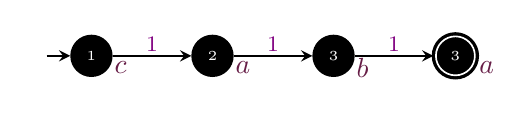
\begin{tikzpicture}[align=center,node distance=1cm]
	\node (init1) {};
	\node[config,right=3mm of init1,label={right,xshift=-1mm,yshift=-1.5mm}:\tcolor$c$] (s1) {1};
	\node[config,right=of s1,label={right,xshift=-1mm,yshift=-1.5mm}:\tcolor$a$]       (s2) {2};
	\node[config,right=of s2,label={right,xshift=-1mm,yshift=-1.5mm}:\tcolor$b$]       (s3) {3};
	\node[config,accepting,right=of s3,label={right,xshift=-1mm,yshift=-1.5mm}:\tcolor$a$]       (s4) {3};
	
	\draw[link] (init1) -- (s1);
	\draw[link] (s1) -- node[font=\footnotesize,yshift=1.5mm] {\pcolor$1$} (s2);
	\draw[link] (s2) -- node[font=\footnotesize,yshift=1.5mm]{\pcolor$1$} (s3);
	\draw[link] (s3) -- node[font=\footnotesize,yshift=1.5mm]{\pcolor$1$} (s4);
	\end{tikzpicture}
\end{document}



%
%
%\documentclass[tikz]{standalone}
%
%\tikzstyle{node}=[draw=#1,fill=#1!20]
%
%\newcommand{\vertex}[6]{\node[shape=circle,fill=black, scale=0.5,label=#1:{#2},label=#5:{\tiny\texttt{\color{blue}#6}},#4] (#3)  {};}
%\newcommand{\myedge}[4]{ \draw[->] (#1) edge node[#2] {#3} (#4);}
%\usetikzlibrary{automata}
%\tikzset{
%	initial text=\(\ast\),
%}
%
%\begin{document}
%\begin{tikzpicture}[align=center,node distance=3cm]
%    % equidistant points and arc
%    \vertex{above}{$\color{green}c$}{s}{initial}{below right}{1}
%    \vertex{above}{$\color{green}a$}{b1}{right of=s}{below right}{2}
%    \vertex{above}{$\color{green}b$}{b2}{right of=b1}{below right}{3}
%    \vertex{above}{$\color{green}a$}{b}{right of=b2,accepting,state,scale=0.4}{below right}{4}
%    
%        \myedge{s}{above}{$\scriptscriptstyle{\color{red}1}$}{b1}
%    \myedge{b1}{above}{$\scriptscriptstyle{\color{red}1}$}{b2}
%    \myedge{b2}{above}{$\scriptscriptstyle{\color{red}1}$}{b}
%
%\end{tikzpicture}
%
%\end{document}
